\documentclass[tikz,border=3pt]{standalone}
\usetikzlibrary{shapes.geometric}
% \usetikzlibrary{arrows.meta}
\usetikzlibrary{decorations.text}
\definecolor{mygray}{RGB}{143,188,143}
\definecolor{boxgray}{RGB}{200,200,200}

\definecolor{testblue}{RGB}{200,200,200}
\definecolor{designyellow}{RGB}{200,200,200}

\definecolor{darkgreen}{RGB}{0,100,0}
\newcommand*{\mytextstyle}{\sffamily\Large\bfseries\color{black!85}}

\newcommand*{\boxtextstyle}{\sffamily\small\bfseries\color{black!85}}

\begin{document}
\begin{tikzpicture}[square/.style={regular polygon,regular polygon sides=4}]
    
    \node[fill=gray!20, text width = 7cm,draw=black]  at (-1,3.5)[
      font  = \boxtextstyle,
      align = left](design)
      {Design deltas - reusable, inheritable changes};
    
    \node[fill=blue!20, text width = 3cm,draw=black]  at (-3,2.5)[
      font  = \boxtextstyle,
      align = left](design)
      {Wild-type strain};
    
    \node[fill=red!20, text width = 3cm, draw=black]  at (3, 2.5) [
      font  = \boxtextstyle,
      align = left] (learn) {Knock-out strain};
    
    \node[fill=green!20, text width = 3cm, draw=black]  at (9, 2.5) [
      font  = \boxtextstyle,
      align = left] (learn) {Production strains};
    
    %design
    
    
    \node at (-3,0) {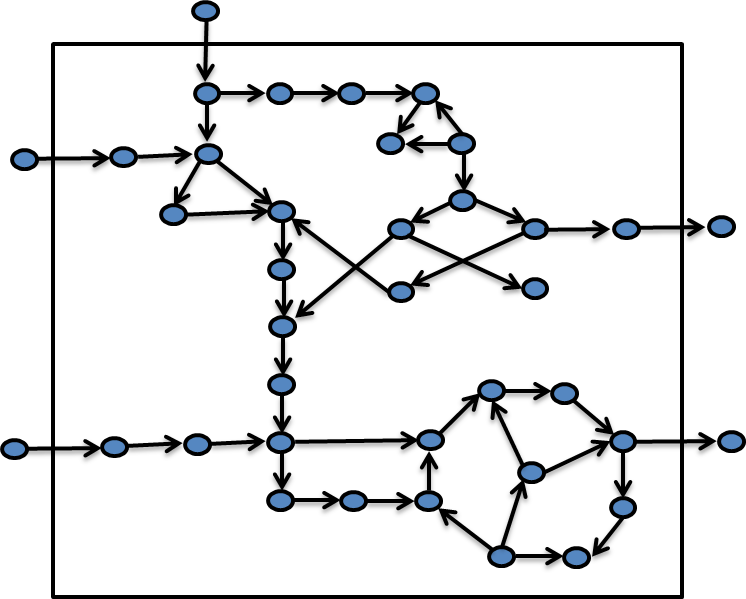
\includegraphics[width=4cm]{model.png}};

    \node at (3,0) {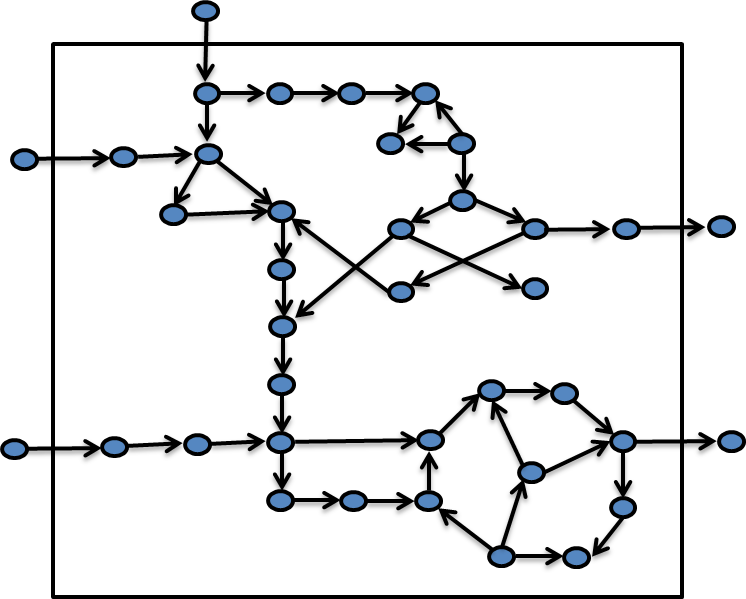
\includegraphics[width=4cm]{model.png}};
    
    \node at (3.65,0.3) {
\includegraphics[width=0.25cm]{cross.png}};
    \node at (2.9,-0.74) {
\includegraphics[width=0.25cm]{cross.png}};
    
    \node at (9,0) {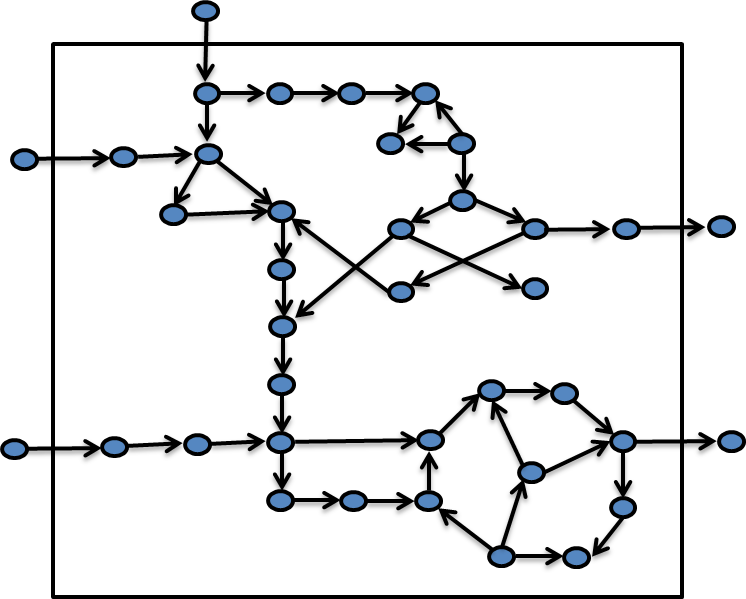
\includegraphics[width=4cm]{model.png}};
    
    \node at (9.65,0.3) {
\includegraphics[width=0.25cm]{cross.png}};
    \node at (8.9,-0.74) {
\includegraphics[width=0.25cm]{cross.png}};
   
    \node at (9.1,-1.5) {\includegraphics[width=0.9cm, angle=300]{pathway.eps}};
   
    \node at (9,-4) {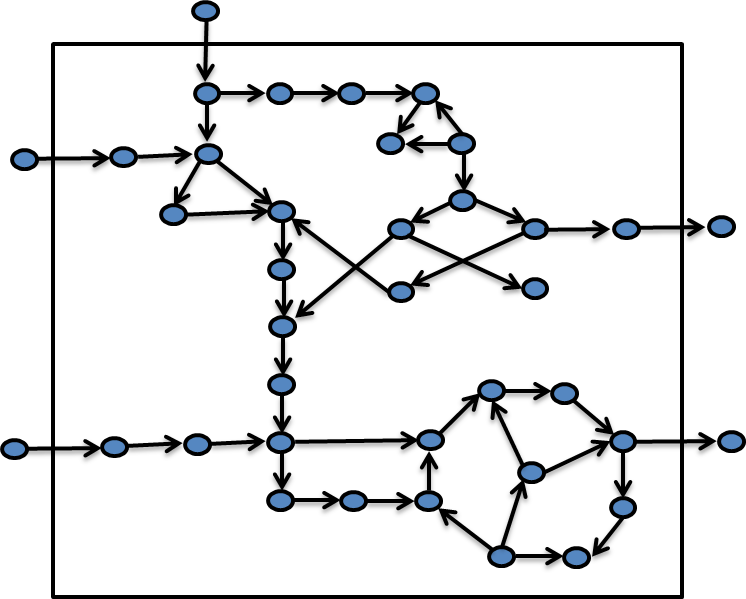
\includegraphics[width=4cm]{model.png}};
     \node at (9.1,-5.5) {\includegraphics[width=0.9cm, angle=300]{pathway.eps}};
   
    \path [->,very thick]  (-1, 0 ) edge (1, 0);
    
    \node [fill=gray!20] (CRA) at (0,0.4) {
\includegraphics[width=0.25cm]{cross.png} 
\includegraphics[width=0.25cm]{cross.png}};
   
    \path [->,very thick]  (5, 0 ) edge (7, 0);
    
    \node [fill=gray!20]  at (6,0.4) {
\includegraphics[width=0.25cm]{cross.png} 
\includegraphics[width=0.25cm]{cross.png}};
    
    \node [fill=gray!20] (PA) at (6,-0.4) {\includegraphics[width=1cm]{pathway.eps}};

    \path [-,very thick]  (-3, -2) edge (-3, -4.02);
    
    \node [fill=gray!20] (PB) at (6,-3.6) {\includegraphics[width=1cm]{pathway.eps}};
    \path [->,very thick]  (-3, -4 ) edge (7, -4);
    
        
    \node[fill=gray!20, text width = 6.5cm,draw=black]  at (1,-5)[
      font  = \boxtextstyle,
      align = left](dbox)
      {Only store differences: \\ Relate changes to real strains};
   
   \node [fill=gray!20] at (3.6,-5) {\includegraphics[width=1cm]{pathway.eps}};
   \node [fill=gray!20] at (2.4,-5) {
\includegraphics[width=0.25cm]{cross.png}};
   \node [fill=gray!20] at (2.8,-5) {
\includegraphics[width=0.25cm]{cross.png}};

\end{tikzpicture}
\end{document}
